\chapter{ML2P-VAE Results and Discussion}

The ML2P-VAE method has been used in a various settings in multiple publications \cite{ijcnn_paper, aied_paper, ml_paper}. The first paper introduced the method and gives some preliminary results on a small simulated data set. The second, a follow-up presented at the Conference for Aritificial Intelligence in Education, displays the advantages that a VAE holds over a regular autoencoder in the task of parameter estimation. The final publication, which has been submitted to Machine Learning, compares different variations of ML2P-VAE with traditional parameter estimation methods on both real and simulated data sets of various sizes.

\section{Description of Data Sets}
\subsubsection*{Sim-ECPE} This simulated data set is designed to mirror the real-life Examination for the Certificate of Proficiency in English, detailed further in the next description. Sim-ECPE has 28 items assessing 3 latent traits. Values for the item parameters in the ML2P model were generated from a uniform distribution so that $a_{ik} \in [0.25, 1.75]$ and $b_i \in [-3,3]$. The range for the discrimination parameters was chosen such that $0.25 \leq MDISC_i \leq 1.75$ \sideremark{Define MDISC} for all $i$. Up to 10,000 student abilities $\Theta \in \R^3$ were sampled from $\mathcal{N}(0,I)$. Note that in Sim-ECPE, it is assumed that the latent traits are independent. We use a $Q$-matrix consistent with previous literature \cite{daSilva2018, Templin2013, henson2007}.

\subsubsection*{ECPE} The Examination for the Certificate of Proficiency in English (ECPE) is an exam with 28 items. The set of responses we use is available in the \textbf{CDM} package for R \cite{cdm}. This includes 2,922 students and a $Q$-matrix for three skills - ``morphosyntactic rules'', ``cohesive rules'', and ``lexical rules''. Since this is a real-world data set, there are not ``true'' values of item or student ability parameters to compare with the model estimates.

\subsubsection*{Sim-6} A moderately-sized simulated data set, Sim-6 has 50 items evaluating 6 latent traits. The $Q$-matrix is also generated randomly, where each entry $q_{ki}$ is sampled from $\text{Bern}(0.2)$. To ensure each item requires at least one latent ability, if a column $q_{:i} = 0$ after sampling, then one random element in the column is changed to a 1. The discrimination parameters are chosen so that $a_{ik} \in [0.1, 1.3]$ and $b_i \in[-3,3]$. Abilities $\Theta \in \R^6$ of 20,000 students were sampled from $\mathcal{N}(0, \Sigma)$, where $\Sigma$ is a correlation matrix with all positive values generated using the SciPy package \cite{SciPy}.

\subsubsection*{Sim-20} This large data set is generated in a similar manner to Sim-6, but includes 50,000 students, 200 items, and 20 latent traits. The $Q$-matrix was generated in the exact same was as that of Sim-6, where $q_{ki} \sim \text{Bern}(0.2)$. The difficulty parameters were sampled uniformly so that $b_i \in [-3,3]$, and the discrimination parameters were sampled uniformly so that $a_{ik} \in [0.1, 0.9]$. As in Sim-6, the 20 latent abilities are correlated with one another, and the correlation matrix is generated in the same manner.

\section{Quantitative Results}

\subsection{Preliminary Results}\label{sec:prelim}
IJCNN

\subsection{Ablation Study}
This could be helpful

\subsection{Variational Autoencoder vs Autoencoder}
\sideremark{AIED}
Shortly after introducing the ML2P-VAE method, comparisons between a variational autoencoder (VAE) and a regular autoencoder (AE) for parameter estimation were made \cite{aied_paper}. Recall that Guo et al. proposed a neural network approach to estimating student mastery in 2017 \cite{guo2017}. This neural network had autoencoding structure, but was geared towards CDM and did not make a connection to IRT or parameter estimation. In this section, we show empirically that using a VAE produces better item and ability estimates than a regular autoencoder and analyze the differences in models leading to this imporvement.

For these experiments, the same simulated data presented in Section \ref{sec:prelim} is used here. The neural architecture used for all experiments includes 28 input/output nodes (one for each item), one hidden layer in the encoder with 10 nodes, and an encoded dimension of 3, representing three latent traits. The decoder has no hidden layers, with connections determined by a given $Q$-matrix. Of course, the VAE includes three extra nodes in the encoder output representing variance so that the VAE encoder produces a standard normal distribution.

\begin{table}[h]
\centering
\begin{tabular}{cccccc}
\hline
Model   & $a_1$ & $a_2$ & $a_3$ & $b$ & Statistic \\
\hline
AE & 0.680 & 0.227 & 0.529 & 2.305 & AVRB \\
VAE   &0.284  & 0.159 & 0.264 & 1.894 &  \\
\hline
AE & 0.585 & 0.481 & 0.534 & 1.651 & RMSE \\
VAE   & 0.322 & 0.346 & 0.264 & 1.670 & \\
\hline
AE & 0.529 & 0.547 & 0.748 & 0.917 & CORR \\
VAE   & 0.924 & 0.920 & 0.986 & 0.990 & \\
\hline
\end{tabular}
\caption{Statistics for item parameter recovery.}
\label{tab:vae_vs_ae_items}
\end{table}

Three error measures for VAE and AE estimates are given in Table \ref{tab:vae_vs_ae_items} and Table \ref{tab:vae_vs_ae_theta}. These include absolute value relative bias (AVRB), root mean square error (RMSE) and Pearson correlation (CORR). The statistics for item parameter estimates in Table \ref{tab:vae_vs_ae_items}, where $a_k$ denotes the average measure taken over all items related to latent trait $\theta_k$, and $b$ is the average measure taken over all item difficulty parameters. Note that the AVRB values for difficulty parameters is rather high, likely due to some of the true values of $b_i$ are very near zero. The item parameter estimates from VAE outperform those from AE for each category and measure. This is corroborated by the correlation plots in Figure \ref{fig:vae_vs_ae_a} and Figure \ref{fig:vae_vs_ae_b}.

\begin{figure}[h!]
\minipage{0.5\textwidth}
   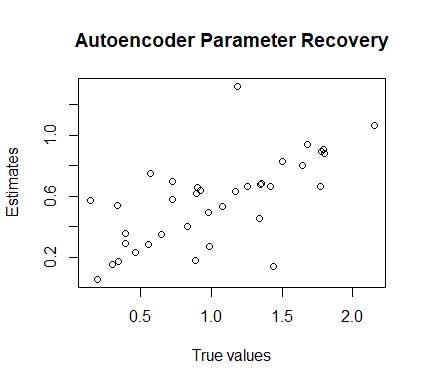
\includegraphics[width=\textwidth]{img/aied_results/ae_a_corr.png}
   \endminipage\hfill
   \minipage{0.5\textwidth}
   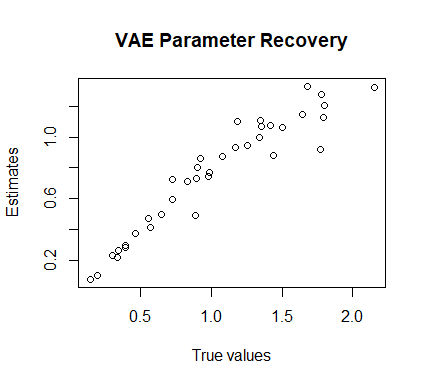
\includegraphics[width=\textwidth]{img/aied_results/vae_a_corr.png}
   \endminipage\hfill
   \caption{Autoencoder and VAE discrimination parameter ($a_{ji}$) recovery.}
   \label{fig:vae_vs_ae_a}
\end{figure}


\begin{figure}[h!]
\minipage{0.5\textwidth}
   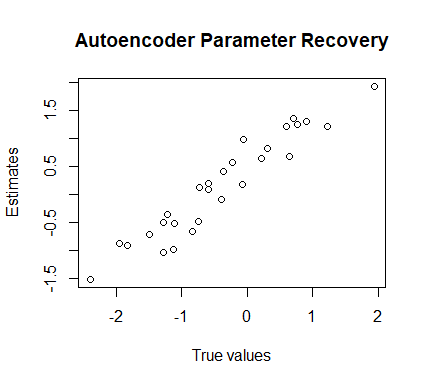
\includegraphics[width=\textwidth]{img/aied_results/ae_b_corr.png}
   \endminipage\hfill
   \minipage{0.5\textwidth}
   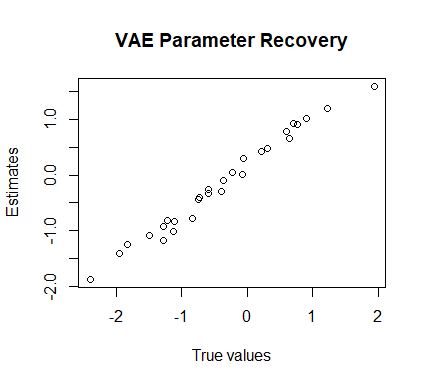
\includegraphics[width=\textwidth]{img/aied_results/vae_b_corr.png}
   \endminipage\hfill
   \caption{Autoencoder and VAE difficulty parameter ($b_i$) recovery.}
   \label{fig:vae_vs_ae_b}
\end{figure}

Results for student ability parameter estimates are shown in Table \ref{tab:vae_vs_ae_theta} and Figure \ref{fig:vae_vs_ae_theta}. Again, we see that the error measures from VAE estimates are much lower than those from AE. However, the correlation values are slightly better for AE, though the difference is not visible in the correlation plot. The reason that AE has poor error measures yes good correlation is because the ability parameter estimates are on a different scale than the true values. Notice in the left plot of Figure \ref{fig:vae_vs_ae_theta} that the vertical axis is on a different scalethan that of the right plot. This is likely due to the fact that a VAE has a KL-divergence term in its loss function.

\begin{table}[h!]
\centering
\begin{tabular}{ccccc}
\hline
Model & $\theta_1$ & $\theta_2$ & $\theta_3$ & Statistic \\
\hline
AE &  7.425 & 3.107 & 16.260 & AVRB \\
VAE   & 1.844 & 1.713 & 4.009 &  \\
\hline
AE & 1.788 & 1.523 & 1.746 & RMSE \\
VAE   & 0.664 & 0.760 & 0.646 & \\
\hline
AE & 0.970 & 0.937 & 0.971 & CORR \\
VAE   & 0.965 & 0.940 & 0.969 & \\
\hline
\end{tabular}
\caption{Statistics for latent trait prediction.}
\label{tab:vae_vs_ae_theta}
\end{table}

The lack of a KL-divergence term in an AE also helps explain the poor discrimination parameter estimates shown in the right plot of Figure \ref{fig:vae_vs_ae_a}. The ML2P model can suffer from an identifiability issue without the assumption that student ability parameters follow some probability distribution \cite{ets2005}. Adding a KL-divergence term in the VAE loss function between the encoder output and the prior $p(\theta)$, which is $\mathcal{N}(0,I)$ in this case.

\begin{figure}[h!]
\minipage{0.5\textwidth}
   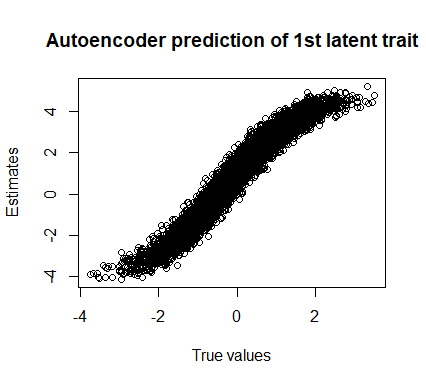
\includegraphics[width=\textwidth]{img/aied_results/ae_theta1_corr.png}
   \endminipage\hfill
   \minipage{0.5\textwidth}
   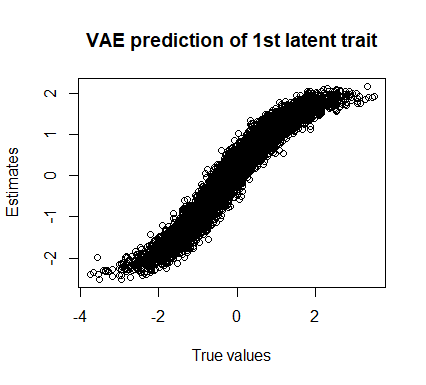
\includegraphics[width=\textwidth]{img/aied_results/vae_theta1_corr.png}
   \endminipage\hfill
   \caption{Autoencoder and VAE predictions for $\theta_1$.}
   \label{fig:vae_vs_ae_theta}
\end{figure}

Both autoencoders and variational autoencoders can be used as IRT parameter estimation methods when a $Q$-matrix restricts weights in the decoder. In either case, adding interpretability to neural networks is interesting, but a VAE is able to incorporate an extra piece of domain knowledge in the prior distribution of $\Theta$, leading to more accurate estimates.


\subsection{ML2P-VAE vs Traditional Methods}
\sideremark{TODO: do 1pl in mirt and VAE}
In this section, a direct comparison of ML2P-VAE with traditional parameter estimation techniques for IRT. Three variants of ML2P-VAE are used: ML2P-VAE$_{full}$, ML2P-VAE$_{est}$, and ML2P-VAE$_{ind}$ as described in Section \ref{sec:variants}. These are compared against Metropolis-Hastings Robbins-Monro (MHRM) \cite{cai2009}, Quasi Monte-Carlo Expectation Maximization (QMCEM) \cite{mirt}, and Monte-Carlo Expectation Maximization (MCEM) \cite{bock1981}. This work has been submitted to the Machine Learning journal \cite{ml_paper}. \sideremark{update if this ever gets accepted}

A summary of each method's performance is given in Table \ref{tab:ml2p_results}. All experiments were conducted using Tensorflow for R on a laptop computer with a 2.9 GHz Intel Core i7-7500U CPU. The results from traditional methods were obtained using default settings of the MIRT package \cite{mirt}. 
In all variations of ML2P-VAE, we train the neural network with the ADAM optimizer for 10 epochs and batch size 1 (pure stochastic gradient descent). The regularization parameter in Equation \ref{vae_loss} \sideremark{fix reference} was fixed  at $\lambda=1$. The specific encoder architecture of the neural network was dependent on the size of the data set. Sim-6 used two hidden layers of size 32 and 16, ECPE used two hidden layers of 16 and 8 nodes, and Sim-20 utilized two hidden layers of size 64 and 32. In each network, a sigmoidal activation function was used in the encoder hidden layers and a linear activation function in the encoded distribution. As described earlier, the ML2P-VAE model requires the use of a sigmoidal activation function in the output layer of the decoder.

\begin{sidewaystable}
\footnotesize{
\centering
\begin{tabular}{c|c|ccc|ccc|ccc|c}
    Data Set & Method & $a$.RMSE & $a$.BIAS & $a$.COR & $b$.RMSE & $b$.BIAS & $b$.COR &  $\theta$.RMSE & $\theta$.BIAS & $\theta$.COR & Runtime \\
    \hline
& MHRM & 0.0693 & 0.0319  & 0.9986   & 0.0256 & -0.0021 & 0.9999  & 0.714  & -0.0033  & 0.7006 & 1110s \\ 
(i)& QMCEM & 0.149 & -0.067 & 0.9939 & 0.0376 & -0.002 & 0.9998 & 0.7206 & 0.0023 & 0.6939 & 322s\\
6 abilities& MCEM & 0.1497 & -0.0633 &  0.9936 &  0.0383 & 0.0035 & 0.9997 &  0.7206 & -0.0016 & 0.6938 & 1009s\\
Sim-6& ML2P-VAE$_{full}$ & 0.0705 &  0.0255  & 0.9985   & 0.0471 & -0.0079 & 0.9996  & 0.6649   & -0.0178  & 0.7476 & 343s\\
& ML2P-VAE$_{est}$ & 0.1803 & 0.0871  & 0.9891 &  0.064 & -0.0131 & 0.9993  & 0.7109 &  0.0772  & 0.7082 & 364s \\
& ML2P-VAE$_{ind}$ & 0.1218 & -0.0004 & 0.9944   & 0.0597 & -0.0145 & 0.9994  & 0.7222 &  0.0316  & 0.6928 & 252s\\
\hline 
& MHRM* & 0* & 0*&  1* &  0* &  0* &  1* & 0* & 0* &  1* & 162s \\
(ii)& QMCEM & 0.0159  & 0.0035 & 0.9999 & 0.0067  & -0.0005 & 1   & 0.0111 & 0.0007 & 0.9999 & 192s\\
3 abilities & MCEM & 0.0228 & 0.0148 & 0.9998 & 0.0064  & -0.0008 & 1   & 0.0132 & 0.0026 & 0.9998 & 33s \\
ECPE & ML2P-VAE$_{full}$ & N/A & N/A & N/A & N/A & N/A & N/A & N/A & N/A & N/A & N/A  \\
& ML2P-VAE$_{est}$ & 0.2794 & 0.2152 & 0.9713 & 0.148 & 0.0951  & 0.993 & 0.443 & -0.0628 & 0.8237 & 61s  \\
& ML2P-VAE$_{ind}$ & 0.3208 & 0.2184 & 0.9504 & 0.154 & 0.0872  & 0.9932  & 0.3063 & 0.01 & 0.9017 & 49s \\
\hline
& MHRM & N/A & N/A & N/A & N/A & N/A & N/A & N/A & N/A & N/A & N/A  \\
(iii)& QMCEM & N/A & N/A & N/A & N/A & N/A & N/A & N/A & N/A & N/A & N/A \\
20 abilities & MCEM & N/A & N/A & N/A & N/A & N/A & N/A & N/A & N/A & N/A & N/A  \\
Sim-20 & ML2P-VAE$_{full}$ & 0.078 &  0.0473  & 0.9983  & 0.0608 &  0.0054  & 0.9996  & 0.6145 &  0.0065  & 0.7893 & 1292s \\
& ML2P-VAE$_{est}$ & 0.2992  & -0.1304  & 0.9822  & 0.1655 &  0.1215  & 0.9987  & 0.7364   & -0.0276  & 0.7257 & 961s \\
& ML2P-VAE$_{ind}$ & 0.2043 &   0.0592  & 0.9792  & 0.0958   & -0.0029  & 0.9992  & 0.7054 &  0.0747  & 0.7135 & 850s \\
\hline
\end{tabular}
\caption{Error measures for discrimination ($a$), difficulty ($b$), and ability ($\theta$) parameters from various parameter estimation methods on three different data sets. Note that in the ECPE data set, there are no true values, so MHRM estimates are accepted as true. In Sim-20, only ML2P-VAE methods are capable of estimating such high-dimensional latent traits}
  \label{tab:ml2p_results}
}
\end{sidewaystable}

Note that when comparing error measures in Sim-6, the ML2P-VAE methods are competitive with traditional methods. In particular, assuming full knowledge of the latent trait covariances in ML2P-VAE yields discrimination, difficulty, and ability parameter estimates of similar accuracy to MHRM. When the assumption of known latent trait correlation is relaxed, the accuracy of parameter estimates understandably slip.

Although the ML2P-VAE methods are slightly less accurate than MHRM, they are much faster than traditional methods, especially as the number of latent traits increase. Much of this speedup is due to the fact that neural networks do not require numerical integration over the latent abilities. While quadrature or MCMC methods become infeasible on data sets much larger than Sim-6, this is no cause for concern with ML2P-VAE. Note that for neural networks of this size (50-200 inputs and latent dimension 6-20), the longer runtime is more due to the number of data samples, rather than the size of the latent dimension. In fact, the largest neural network we used in these experiments, used on Sim-20, only had 1,670 trainable parameters, which is very small when compared to ANN used for image classification. 

\begin{figure}[h]
\centering
\figuretitle{Discrimination Parameter Estimates}\\
    \begin{subfigure}{.32\textwidth}
      \centering
      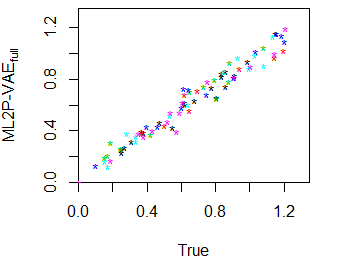
\includegraphics[width=.9\linewidth]{img/ml_journal_results/6skills/vae_full_disc_6skills.png}
    \end{subfigure}
    \begin{subfigure}{.32\textwidth}
      \centering
      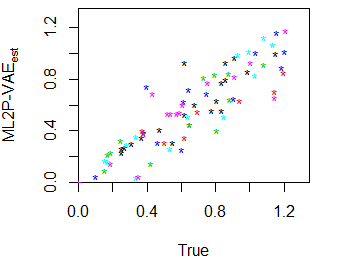
\includegraphics[width=.9\linewidth]{img/ml_journal_results/6skills/vae_est_disc_6skills.png}
    \end{subfigure}
    \begin{subfigure}{.32\textwidth}
      \centering
      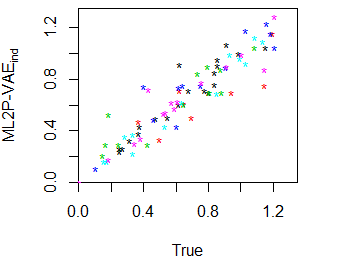
\includegraphics[width=.9\linewidth]{img/ml_journal_results/6skills/vae_ind_disc_6skills.png}
    \end{subfigure}
    \begin{subfigure}{.32\textwidth}
      \centering
      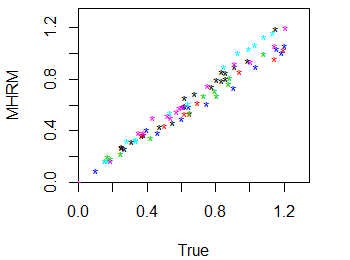
\includegraphics[width=.9\linewidth]{img/ml_journal_results/6skills/mhrm_disc_6skills.png}
    \end{subfigure}
    \begin{subfigure}{.32\textwidth}
      \centering
      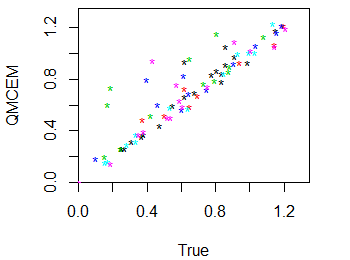
\includegraphics[width=.9\linewidth]{img/ml_journal_results/6skills/qmcem_disc_6skills.png}
    \end{subfigure}
    \begin{subfigure}{.32\textwidth}
      \centering
      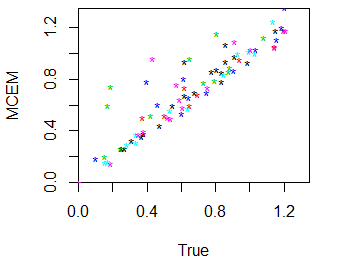
\includegraphics[width=.9\linewidth]{img/ml_journal_results/6skills/mcem_disc_6skills.png}
    \end{subfigure}
    \caption{Correlation plots of discrimination parameter estimates for the Sim-6 dataset with 50 items and 6 latent traits. ML2P-VAE estimates are on the top row, and traditional method estimates are on the bottom row}
    \label{fig:6skill_cor}
\end{figure}

Some of the results are visualized in Figures \ref{fig:6skill_cor}, \ref{fig:ecpe_cor}, and \ref{fig:20skill_cor} for Sim-6, ECPE, and Sim-20, respectively. Figure \ref{fig:6skill_cor} shows the correlation between the true and estimated discrimination parameters for the ML2P-VAE$_{full}$ and MHRM methods. We don't include such plots for the difficultly parameters, as all methods estimate each $b_i$ with very high accuracy. From these figures, it appears that while MHRM obtains better results on smaller discrimination parameters, ML2P-VAE$_{full}$ has less error on larger parameters, and the estimation error seems to be independent of the magnitude of the parameter. The other two ML2P-VAE methods do not obtain the same levels of accuracy as when assuming full knowledge of the latent ability correlations. 

\begin{figure}[h]
\centering
    \begin{subfigure}{.32\textwidth}
      \centering
      \figuretitlesmall{Discrimination Parameters}
      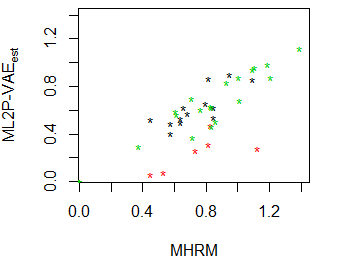
\includegraphics[width=.9\linewidth]{img/ml_journal_results/ecpe/vae_est_disc_ecpe.png}
    \end{subfigure}
    \begin{subfigure}{.32\textwidth}
      \centering
      \figuretitlesmall{Difficulty Parameters}
      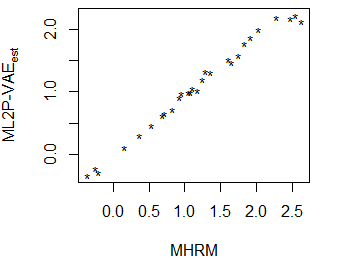
\includegraphics[width=.9\linewidth]{img/ml_journal_results/ecpe/vae_est_diff_ecpe.png}
    \end{subfigure}
    \begin{subfigure}{.32\textwidth}
      \centering
      \figuretitlesmall{Ability Parameters}
      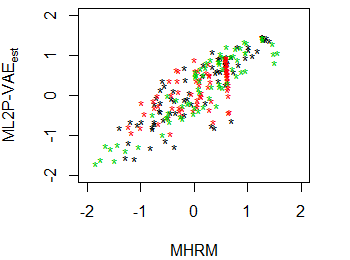
\includegraphics[width=.9\linewidth]{img/ml_journal_results/ecpe/vae_est_theta_ecpe.png}
    \end{subfigure}
    \begin{subfigure}{.32\textwidth}
      \centering
      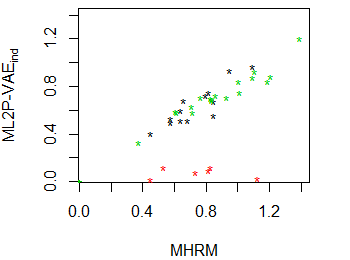
\includegraphics[width=.9\linewidth]{img/ml_journal_results/ecpe/vae_ind_disc_ecpe.png}
    \end{subfigure}
    \begin{subfigure}{.32\textwidth}
      \centering
      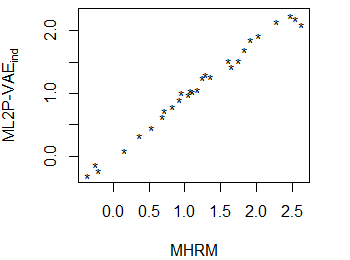
\includegraphics[width=.9\linewidth]{img/ml_journal_results/ecpe/vae_ind_diff_ecpe.png}
    \end{subfigure}
    \begin{subfigure}{.32\textwidth}
      \centering
      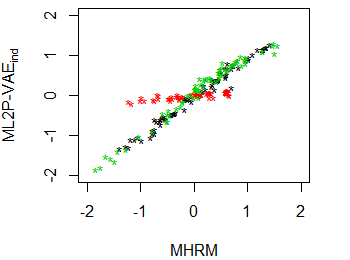
\includegraphics[width=.9\linewidth]{img/ml_journal_results/ecpe/vae_ind_theta_ecpe.png}
    \end{subfigure}
    \caption{Estimates from ML2P-VAE methods plotted against ``accepted'' MHRM estimates from the ECPE dataset}
    \label{fig:ecpe_cor}
\end{figure}

When examining the ECPE data, there are no ``true'' values of parameters, so ML2P-VAE's results are directly compared with MHRM's estimates. As seen in Table \ref{tab:ml2p_results}, the parameter estimates from QMCEM and MCEM are nearly identical to those of MHRM on the ECPE data. Of course, there is not a known covariance matrix between the three latent abilities, so only ML2P-VAE$_{est}$ and ML2P-VAE$_{ind}$ can be analyzed. While both methods perform similar to MHRM in difficulty parameter estimates, we can see that the two yield different results when applied to discrimination and ability parameters. 

First note that while ML2P-VAE$_{ind}$ gives accurate estimations for the green and black abilities (and the discrimination parameters associated with those abilities), the red ability estimates are all very near zero for every student. This tells us that the ML2P-VAE$_{ind}$ method found that the red ability has no effect on exam performance. On the other hand, ML2P-VAE$_{est}$ captures the general trend of the MHRM ability  parameters, but the estimates have much more variance. The discrimination parameter estimates also show some correlation, but each of the three abilities are on a different scale.
\begin{figure}[h]
\centering
\figuretitle{Discrimination and Ability Parameter Estimates}\\
    \begin{subfigure}{.32\textwidth}
      \centering
      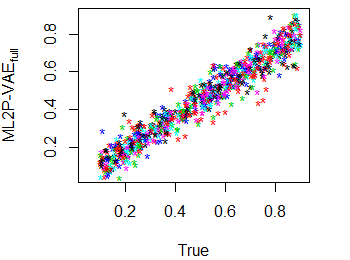
\includegraphics[width=.9\linewidth]{img/ml_journal_results/20skills/vae_full_disc_20skills.png}
    \end{subfigure}
    \begin{subfigure}{.32\textwidth}
      \centering
      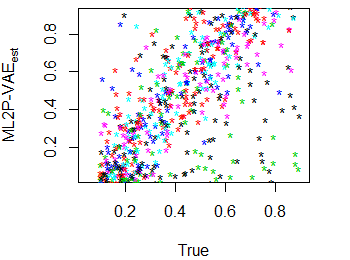
\includegraphics[width=.9\linewidth]{img/ml_journal_results/20skills/vae_est_disc_20skills.png}
    \end{subfigure}
    \begin{subfigure}{.32\textwidth}
      \centering
      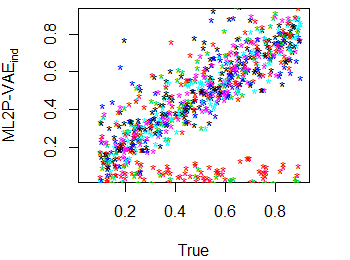
\includegraphics[width=.9\linewidth]{img/ml_journal_results/20skills/vae_ind_disc_20skills.png}
    \end{subfigure}
    \begin{subfigure}{.32\textwidth}
      \centering
      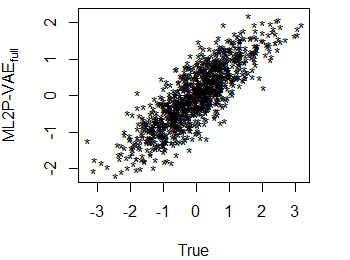
\includegraphics[width=.9\linewidth]{img/ml_journal_results/20skills/vae_full_theta_20skills.png}
    \end{subfigure}
    \begin{subfigure}{.32\textwidth}
      \centering
      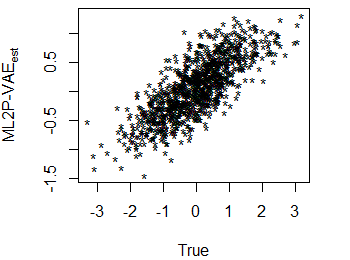
\includegraphics[width=.9\linewidth]{img/ml_journal_results/20skills/vae_est_theta_20skills.png}
    \end{subfigure}
    \begin{subfigure}{.32\textwidth}
      \centering
      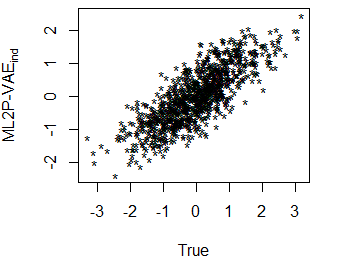
\includegraphics[width=.9\linewidth]{img/ml_journal_results/20skills/vae_ind_theta_20skills.png}
    \end{subfigure}
    \caption{ML2P-VAE parameter estimates for Sim-20 with 200 items and 20 latent traits. The top row shows discrimination parameter correlation, and the bottom row shows ability parameter correlation}
    \label{fig:20skill_cor}
\end{figure}

While estimating parameters for the Sim-20 dataset, the dimension of the latent traits ($\R^{20}$) is too large for traditional methods, so only the three ML2P-VAE techniques are studied. All three of these methods estimate the difficulty parameters with high accuracy. Similar to in Sim-6, it is again observed that the ML2P-VAE$_{full}$ error seems to be independent of the size of the discrimination parameter, a promising trend. However, ML2P-VAE does not perform as well when full knowledge of the latent ability correlation matrix is unknown. The discrimination parameter estimates for ML2P-VAE$_{est}$ seem to have no pattern. Upon closer inspection, it can be seen that the discrimination parameter estimates associated with a particular ability are correlated, but each ability is on a different scale. 

The discrepancy between ML2P-VAE$_{full}$ and ML2P-VAE$_{est}$ can be attributed to a poorly estimated covariance matrix. For this data set, the covariance matrix obtained by the method described previously greatly overestimates every correlation between latent traits: the average signed bias in the correlation matrix estimation is $-0.61$, and even the closest correlation estimation has signed bias $-0.26$. Finding a better method to compute an approximate correlation matrix could greatly improve ML2P-VAE$_{est}$.

The estimates for the Sim-20 dataset produced by ML2P-VAE$_{ind}$ display the same behavior observed in the ECPE dataset. Two of the abilities have discrimination parameters estimated near zero, meaning ML2P-VAE$_{ind}$ deemed these abilities to have no relation with performance on the assessment. But in contrast to the ECPE data, Sim-20 was simulated and so it is known that this is not true. Outside of this issue, the other discrimination parameters were reasonably estimated, showing clear correlation with the true values on near a 1:1 scale.


Though ML2P-VAE$_{est}$ and ML2P-VAE$_{ind}$ have trouble converging to the true discrimination parameters, they are still able to obtain quality estimates to the ability parameters. The values in Table \ref{tab:ml2p_results} for $\theta$ in Sim-20 are comparable to those of Sim-6. The plots in Figure \ref{fig:20skill_cor} show this high correlation in all three ML2P-VAE variants.

\subsubsection{Effect of Training Data Size}
A common criticism of neural networks is that they are computationally intensive and training them with a gradient descent based algorithm (a first order method) can take a long time. They also require large amounts of data. As mentioned before, the architecture used in this application results in a relatively small neural network.

\begin{figure}[h]
\centering
    \begin{subfigure}{.47\textwidth}
      \centering
      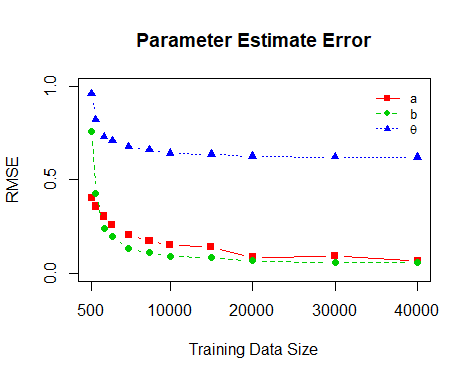
\includegraphics[width=\linewidth]{img/ml_journal_results/vae_full_train_size_error.png}
    %   \caption{}
    %   \label{fig:size_error}
    \end{subfigure}
    \begin{subfigure}{.47\textwidth}
      \centering
      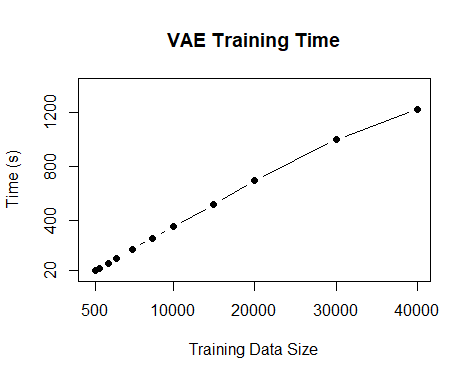
\includegraphics[width=\linewidth]{img/ml_journal_results/vae_full_train_size_time.png}
    %   \caption{}
    %   \label{fig:size_time}
    \end{subfigure}
    \caption{Performance of ML2P-VAE$_{full}$ on data set (iii) when trained on data sets of increasing size. The left plot gives the test RMSE after using different sizes of training data, and the right plot shows the time required to train the neural network}
    \label{fig:train_size}
\end{figure}

The longer runtimes in Table \ref{tab:ml2p_results} for Sim-20 can be attributed more to the fact that there were 50,000 data samples, rather than the large latent dimension. The left plot of Figure \ref{fig:train_size} displays the relation between the size of the training data and estimation accuracy. Error does not decrease very much after the number of training samples becomes greater than 20,000 -- less than half of the available simulated data. The right plot of Figure \ref{fig:train_size} shows that training time grows linearly with the size of training data. 

Both plots in Figure \ref{fig:train_size} demonstrate the trade-off between accuracy and speed, as well as highlighting that ML2P-VAE methods can still be viable even if the data size is not exceptionally large. This is particularly true in estimating the ability parameter $\Theta$, whereas traditional methods are unable to estimate high-dimensional $\Theta$. Estimating the difficulty parameters $b$ is manageable with a smaller data set, while discrimination parameters require a large amount of training data to obtain quality estimates.

\sideremark{could add in some stuff from ML paper Discussion}

%\section{3-PL Results}
\sideremark{am I going to do anything with 3PL?}

